\documentclass[serif,mathserif]{beamer}
\usepackage{etex}
\usepackage{amsmath, amsfonts, epsfig, xspace}
\usepackage{algorithm,algorithmic}
\usepackage{pstricks,pst-node}
\usepackage{multimedia}
\usepackage[normal,tight,center]{subfigure}
\usepackage{beamerthemesplit}
\usepackage{color}
\usepackage{mdframed}
\usepackage{pifont}

\setlength{\subfigcapskip}{-.5em}
\usetheme{lankton-keynote}

\usepackage{graphicx,color}
% remove caption of figure
\usepackage[labelformat=empty]{caption}

\usepackage[none]{hyphenat} % hyphenation is ugly in slides
\usepackage{parskip}

\usepackage{relsize} % \smaller to change size

\usepackage{tikz}
\usetikzlibrary{calc}

\usetikzlibrary{arrows}

\newcommand{\TikzDraw}[2][]{
  \begin{tikzpicture}[overlay, remember picture, shift={(current page.center)}, #1]
    #2
  \end{tikzpicture}
}

\newcommand{\gridlines}{
  \TikzDraw{
    \draw[help lines,xstep=.2,ystep=.2,red!20] (current page.south west) grid (current page.north east);
    \draw[help lines,xstep=1,ystep=1,red] (current page.south west) grid (current page.north east);
    \foreach \x in {-15,-14,...,15} {
      \node [anchor=north, red] at (\x,0) {\tiny \x};
      \node [anchor=east,red] at (0,\x) {\tiny \x};
    }
  }
}

\newcommand{\DrawOnImg}[3][]
{
  \begin{tikzpicture}
    \node[anchor=south west,inner sep=0] (image) at (0,0){
      #2
    };
    \begin{scope}[x={(image.south east)},y={(image.north west)}]
      \ifthenelse{\equal{#1}{grid}}
                 {\draw[color=blue, style=dashed] (0,0) grid[xstep=.1, ystep=.1] (1.0001,1.0001);}
                 {}
                 #3
    \end{scope}
  \end{tikzpicture}
}


\author[Jiong Chen]{Jiong Chen}

\title[\hspace{2em}\insertframenumber/\inserttotalframenumber]{\huge A Chebyshev Semi-Iterative Approach for Accelerating Projective and Position-based Dynamics}

\date{December 29, 2015} %leave out for today's date to be insterted

% \institute{Zhejiang University}

\newcommand{\BOLD}[1]{\mathbf{#1}}
\newcommand{\BOLDG}[1]{\boldsymbol{#1}}
\newcommand{\PDIF}[2]{\frac{\partial #1}{\partial #2}}
\newcommand{\TODO}[1]{\textcolor{red}{#1}}
\newcommand{\TODOB}[1]{\textcolor{blue}{#1}}
\newcommand{\TODOG}[1]{\textcolor{green!50!black}{#1}}
\newcommand{\argmin}{\operatornamewithlimits{arg\min}}
\DeclareMathOperator{\tr}{tr}
\DeclareMathOperator{\cond}{cond}
\DeclareMathOperator{\ST}{s.t.}
\DeclareMathOperator{\diag}{diag}

\newmdtheoremenv{theo}{Theorem}

\definecolor{DARK}{RGB}{45, 33, 73}
\definecolor{LIGHT}{RGB}{119, 52, 106}
\definecolor{TEXTLIGHT}{RGB}{213, 207, 229}
\definecolor{TEXTDARK}{RGB}{66, 66, 66}
\definecolor{BULLET}{RGB}{179, 17, 102}
\definecolor{EM}{RGB}{179,17,102}

\begin{document}

\maketitle

\begin{frame}
 \frametitle{Background}
 \begin{itemize}
  \item Projective dynamics \TODO{\textit{[Bouaziz et al. 2014]}}
  \begin{equation*}
    \BOLD{x}_{t+1}=\argmin_{\BOLD{x}} \frac{1}{2h^2}\|\sqrt\BOLD{M}(\BOLD{x}-\BOLD{s}_t)\|^2+\sum_c\frac{w_c}{2}\|\BOLD{A}_c\BOLD{x}-\BOLD{\hat A}_c\BOLD{q}_c\|^2+\delta_c(\BOLD{q}_c)
  \end{equation*}
  \item Position-based dynamics \TODO{\textit{[M\"uller et al. 2007]}}
    \begin{itemize}
     \item[-] Eliminate $\frac{1}{2h^2}\|\sqrt\BOLD{M}(\BOLD{x}-\BOLD{s}_t)\|^2$
     \item[-] $\BOLD{A}_c = \BOLD{\hat A}_c = \sqrt \BOLD{M}$
     \item[-] Use Gauss-Seidel to solve the global step
    \end{itemize}
 \end{itemize}
\end{frame}

\begin{frame}
 \frametitle{Two Specific Examples}
 \begin{itemize}
  \item Fast mass spring system \TODO{\textit{[Liu et al. 2014]}}
  \begin{equation*}
   \begin{split}
    E(\BOLD{x})=T(\BOLD{x}; \BOLD{x}_t, &\BOLD{v}_t, \BOLD{M}, h)+ \sum_{(i, j)}\frac{w_{i, j}}{2}\|\BOLD{x}_i-\BOLD{x}_j-\BOLD{d}_{i,j}\|^2 \\
    &\ST \quad \|\BOLD{d}_{i,j}\| = r
   \end{split}
  \end{equation*}
  \item Geometric elastic model \TODO{\textit{[Chao et al. 2010]}}
  \begin{equation*}
   \begin{split}
    E(\BOLD{x})=T(\BOLD{x}; &\BOLD{x}_t, \BOLD{v}_t, \BOLD{M}, h)+ \sum_{t}\frac{w_t}{2}\|\BOLD{F}_t-\BOLD{R}_t\|_F^2 \\
    &\ST \quad \BOLD{R}_t \in SO(3)
   \end{split}
  \end{equation*}
 \end{itemize}
\end{frame}

\begin{frame}
 \frametitle{Solvers for Global Step}
 \TikzDraw {
  \node at (-3.3, 0) {\parbox[t]{0.5\textwidth}{
    \begin{itemize}
      \item \textbf{Direct}
      \begin{itemize}
      \item \textit{\TODO{Statble}}
      \item \textit{\TODOG{Relatively expensive}}
      \item \textit{\TODOG{Cannot be accelerated by GPU}}
      \item \textit{\TODOG{Unneeded accuracy}}
      \end{itemize}
      \item \textbf{Jacobi}
      \begin{itemize}
       \item \textit{\TODO{Highly compatible with GPU}}
       \item \textit{\TODOG{Unstatble}}
      \end{itemize}
      \item \textbf{Gauss-Seidel}
    \end{itemize}
  }};
  \node at (2.6, 0) {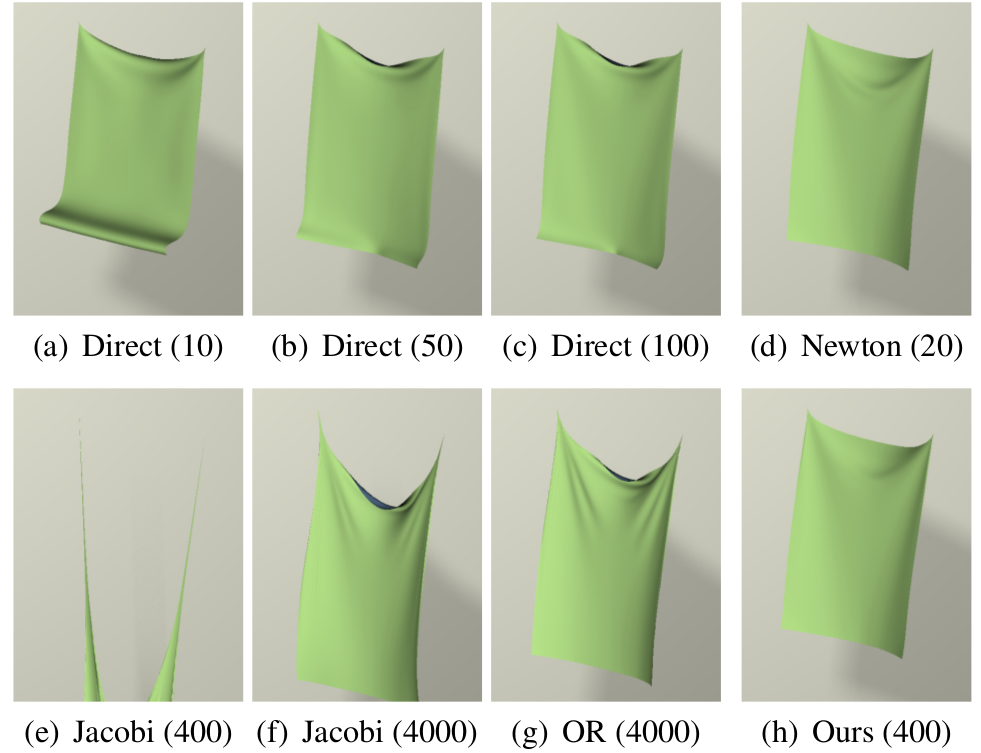
\includegraphics[scale=0.2]{img/diff_ls}};
  \draw[red] (-0.61, 0.82) rectangle (0.5, 1.2);
 }
 %\gridlines
\end{frame}

\begin{frame}
 \frametitle{PD \& Jacobi Method}
 \begin{itemize}
  \item Replace direct solve by one Jacobi iteration.
  \begin{figure}
   \centering
   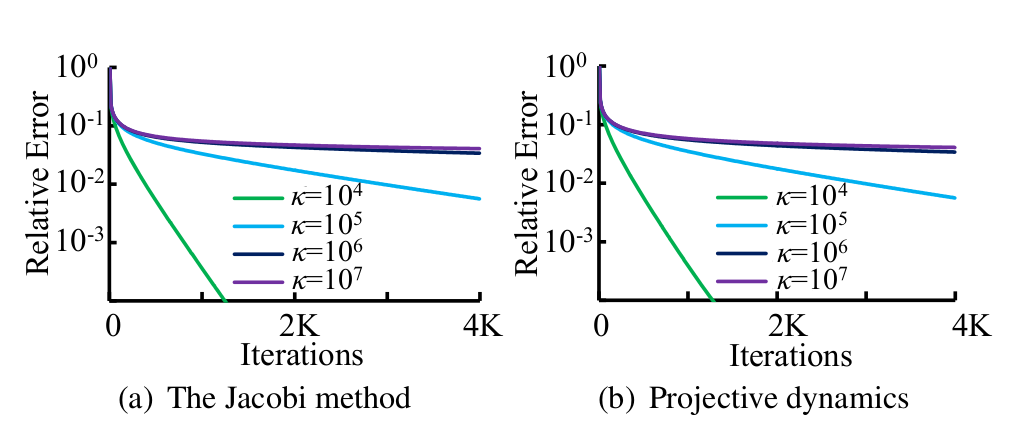
\includegraphics[scale=0.25]{img/conv_comp}
  \end{figure}
  \item \TODO{Explanation: local step is typically stabilized within a few iterations.}
  \item Accelerate convergence $\Rightarrow$ \textbf{Chebyshev semi-iterative approach}.
 \end{itemize}
\end{frame}

\begin{frame}
  \frametitle{Chebyshev Semi-Iterative Approach}
  \begin{itemize}
   \item Jacobi and Gauss-Seidel iteration form:
   \begin{equation*}
   \begin{split}
    \BOLD{x}^{(k+1)} &= \BOLD{B}^{-1}(\BOLD{Cx}^{(k)}+\BOLD{b}) \\
    \BOLD{e}^{(k+1)} &= \BOLD{B}^{-1}\BOLD{Ce}^{(k)} \\
    \BOLD{e}^{(k)} = (&\BOLD{B}^{-1}\BOLD{C})^k\BOLD{e}^{(0)} = \BOLD{Q}\BOLDG{\Lambda}^k\BOLD{Q}^{-1}\BOLD{e}^{(0)}
   \end{split}
   \end{equation*}
  \item Converge $\rho(\BOLD{B}^{-1}\BOLD{C})<1$
  \item Better result by linear combination
  \begin{equation*}
  \begin{split}
   &\BOLD{y}^{(k)} = \sum_{j=0}^k v_{j, k}\BOLD{x}^{(j)} \\
   &\ST \quad \sum_{j=0}^k v_{j, k} = 1
  \end{split}
  \end{equation*}
  \end{itemize}
\end{frame}

\begin{frame}
 \frametitle{Chebyshev Semi-Iterative Approach}
 \begin{itemize}
  \item Error:
  \begin{equation*}
  \begin{split}
   \BOLD{e}^{(k)} &= \BOLD{y}^{(k)}-\BOLD{x}^*=\sum_{j=0}^k v_{j, k}(\BOLD{x}^{(j)}-\BOLD{x}^*) \\
   &= \sum_{j=0}^kv_{j, k}(\BOLD{B}^{-1}\BOLD{C})^j\BOLD{e}^{(0)} = p_k(\BOLD{B}^{-1}\BOLD{C})\BOLD{e}^{(0)}
  \end{split}
  \end{equation*}
  \item Reduce error $\BOLD{e}^{(k)} \Leftrightarrow$ reduce $\|p_k(\BOLD{B}^{-1}\BOLD{C})\|_2 = \max_{\lambda_i}|p_k(\lambda_i)|$
  \item Though $\lambda_i$ is unknown, given spectral radius,
  \begin{equation*}
  \boxed {
  \begin{split}
   p_k(&x) = \argmin { \max_{-\rho \le x \le \rho}|p_k(x)|} \\
    &\Rightarrow \TODO{p_k(x) = \frac{C_k(x/\rho)}{C_k(1/\rho)}}
  \end{split}
  }
  \end{equation*}
 \end{itemize}
\end{frame}

\begin{frame}
 \frametitle{Chebyshev Semi-Iterative Approach}
 \begin{itemize}
  \item Recurrence relation to iterative scheme
  \begin{equation*}
   \begin{split}
    \BOLD{y}^{(k+1)} = &\omega_{k+1}(\BOLD{B}^{-1}(\BOLD{Cy}^{(k)}+\BOLD{b})-\BOLD{y}^{(k-1)})+\BOLD{y}^{(k-1)} \\
    &\omega_{k+1} = \frac{2C_k(1/\rho)}{\rho C_{k+1}(1/\rho)}, i \ge 1, \omega_1 = 1
   \end{split}
  \end{equation*}
  \pause
  \item Looks similar to weighted Jacobi and SOR, but converges much faster.
  \TikzDraw {
    \draw[red] (-2.4, 2.1) rectangle (-1.5, 3.1);
    \draw[red] (3.4, 2.1) rectangle (4.5, 3.1);
  }
  \pause
  \item $\hat \rho$ is the estimated spectral radius.
  \begin{equation*}
   \begin{split}
    \hat \rho &= 0, \text{no acceleration} \\
    \hat \rho &\in (0, \rho], \text{convergence rate} \uparrow \\
    \hat \rho &> \rho, \text{still converges, oscillation happens} \\
    \hat \rho &\rightarrow 1, \text{diverges}
   \end{split}
  \end{equation*}
 \end{itemize}
 %\gridlines
\end{frame}

\begin{frame}
 \frametitle{Chebyshev for PD}
 \TikzDraw {
  \node at (-2.5, 0) {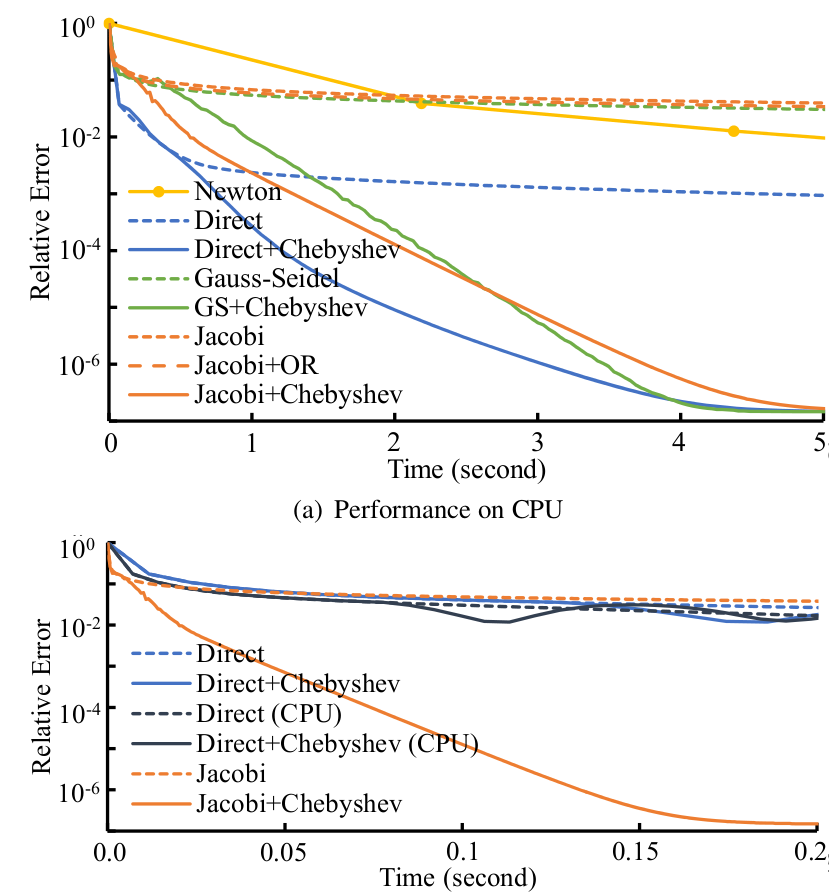
\includegraphics[scale=0.18]{img/performace}};
  \node at (3.2, -0.17) {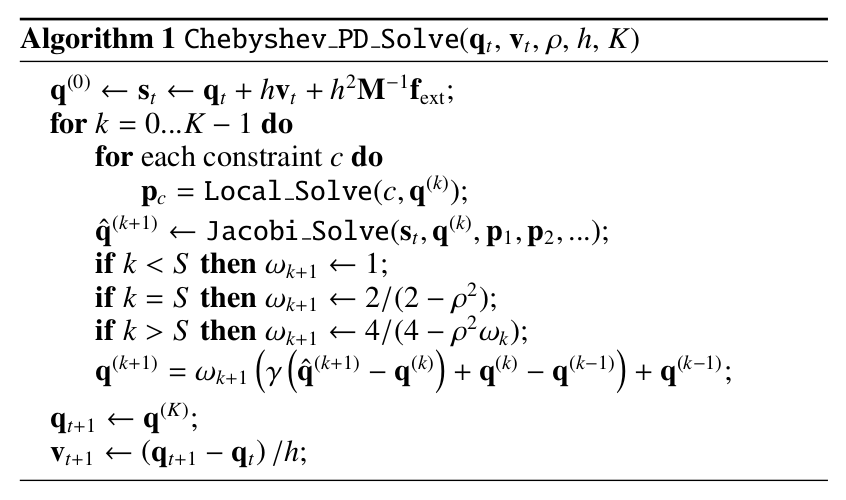
\includegraphics[scale=0.2]{img/algorithm}};
  \draw [fill=white, white] (5.6, -3) rectangle (6.5, 3);
  \visible<2-> {
    \node at (3.2, 2.5) {\TODO{\small also work for direct solve and GS}};
    \draw[->, red] (0.7, 2.25)--(-2.2, 1);
  }
  \visible<3> {
    \node at (3.2, -2.8) {\TODO{\small negligible GPU acceleration for direct}};
    \draw[->, red] (0.7, -2.58)--(-2.0, -1.2);
  }
 }
 %\gridlines
\end{frame}

\begin{frame}
 \frametitle{Issues on Spectral Radius Estimation}
 \begin{itemize}
  \item The choice of $\rho$ via pre-simulation
  \begin{itemize}
   \item Initialize $\rho$ by $\|\BOLD{e}^{(K)}\|_2/\|\BOLD{e}^{(K-1)}\|_2, \BOLD{e}^{(i)} = \nabla E(\BOLD{x}^{(i)})$.
   \item Run the simulation multiple times and manually adjust $\rho$ to maximize convergence rate.
   \item Oscillation occurs$\,\, \Rightarrow \rho \downarrow$.
  \end{itemize}
  \item Experimental conclusions
  \begin{itemize}
   \item $\rho$ is insensitive to state $\BOLD{x}$ and small changes made to system
   \item Object stiffness $\uparrow \,\, \Rightarrow \rho \uparrow$.
   \item Total number of iterations $K \uparrow \,\, \Rightarrow \rho \uparrow$.
  \end{itemize}
 \end{itemize}
\end{frame}

\begin{frame}
 \frametitle{Issues on Convergence\&Robustness}
 \begin{itemize}
  \item Divergence issue I
  \begin{itemize}
    \item $i \uparrow$, convergence rate drops quickly \& Use constant $\rho$.
    \item When $K$ is large, $\rho$ is over-estimated for first few iterations.
    \item Fix strategy: \ding{182}~\TODO{delay Chebyshev;} \ding{183} \TODOG{variant $\rho$.}
  \end{itemize}
  \item[]
  \item Divergence issue II
  \begin{itemize}
   \item Jacobi iteration:\quad $\rho(\BOLD{B}^{-1}\BOLD{C}) < 1$
   \item Fix strategy: \ding{182} \TODO{under-relaxation step;} \ding{183} \TODOG{strain limiting.} 
   \begin{equation*}
   \begin{split}
    \BOLD{x}^{k+1} = \omega_{k+1}(&\TODO{\gamma(\hat{\BOLD{x}}^{(k+1)}-\BOLD{x}^{(k)})+\BOLD{x}^{(k)}}-\BOLD{x}^{(k-1)})+\BOLD{x}^{(k-1)} \\
    &\gamma \in [0.6, 0.9]
   \end{split}
   \end{equation*}
  \end{itemize}
 \end{itemize}
 \TikzDraw {
  \node at (3.6, -0.28) {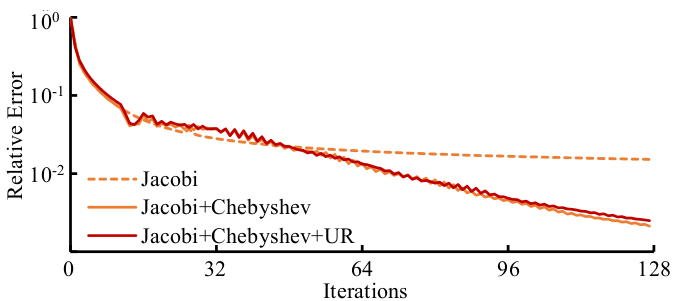
\includegraphics[scale=0.2]{img/UR}};
  \draw[red, thick] (-1.2, -0.8) -- (1, -1.02);
 }
 %\gridlines
\end{frame}

\begin{frame}
 \frametitle{Reproduced Results Summary}
  Direct+Chebyshev \& One Jacobi+Chebyshev
  \begin{itemize}
    \item \TODO{The estimation of $\rho$ has significant impact on the convergence.}
    \item $\rho_{tet}(0.87375) < \rho_{spring}(0.9992)$
    \TikzDraw {
      \visible<2> {
	\node at (-2.5, -1.3) {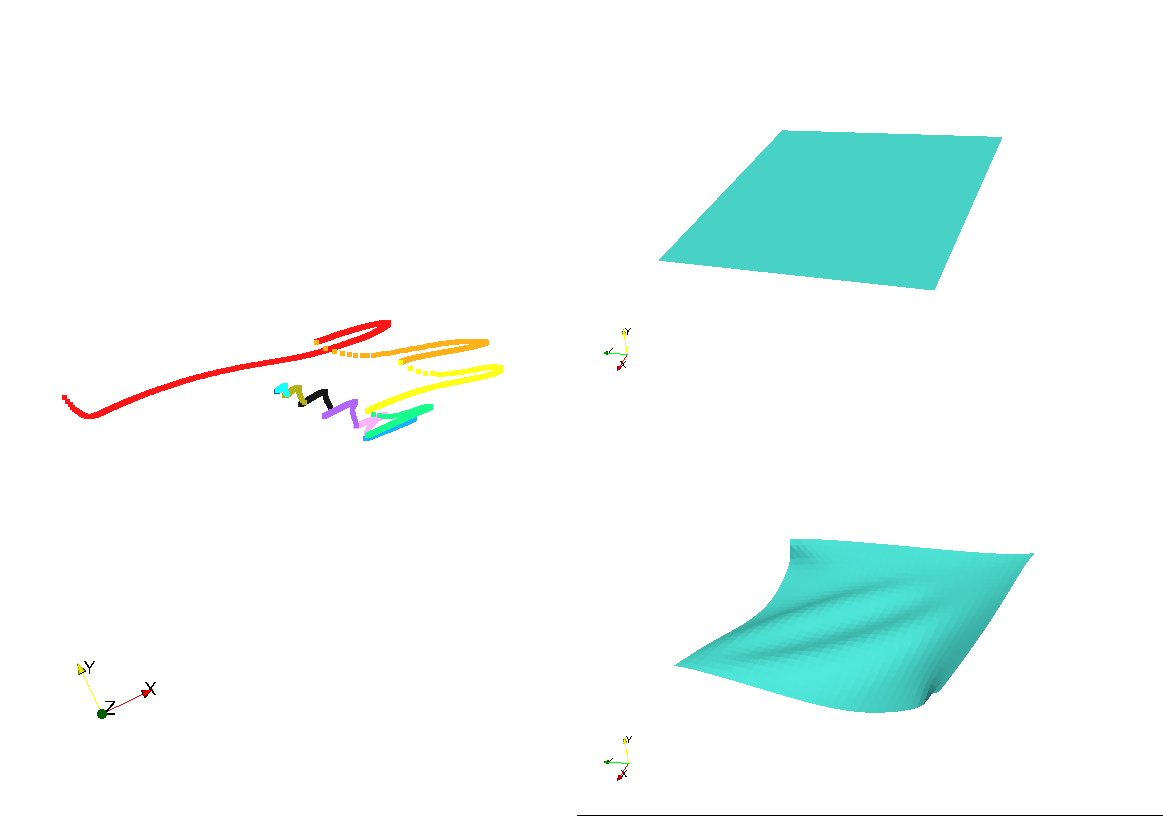
\includegraphics[scale=0.12]{img/mass_spring_rot}};
	\node at (2, -1.3) {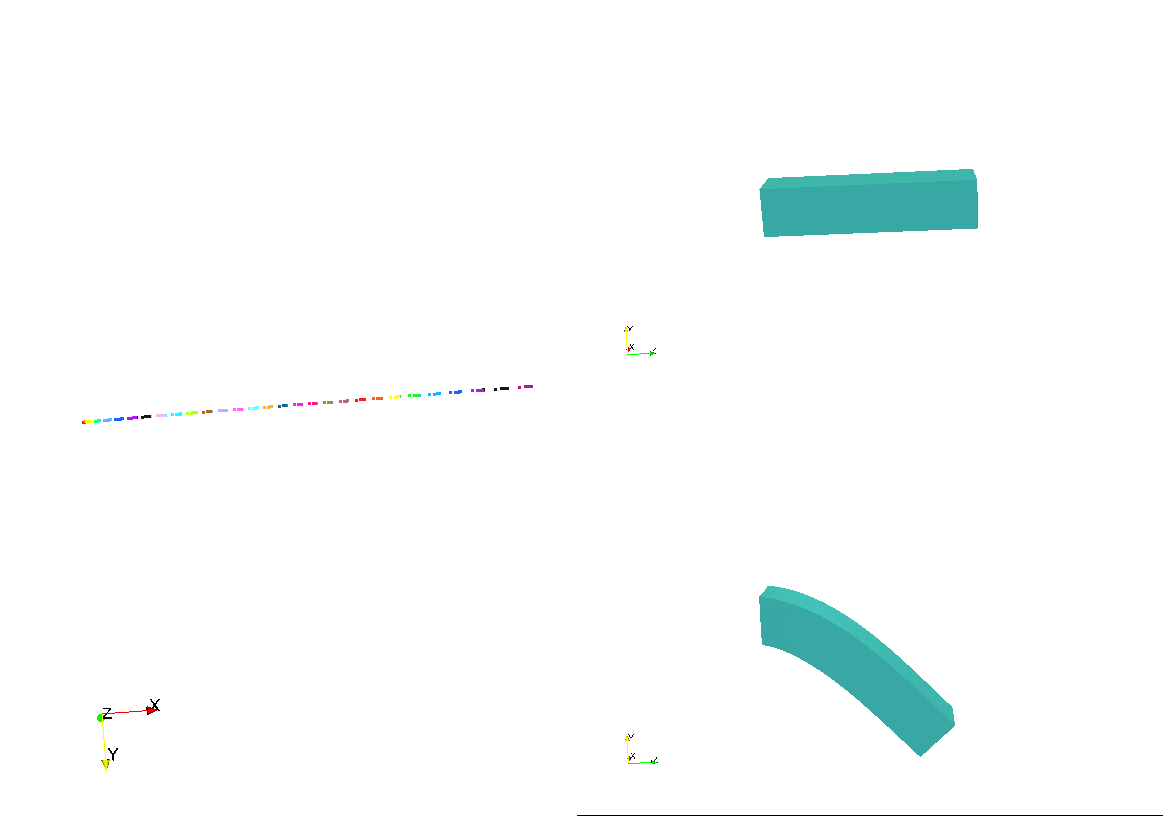
\includegraphics[scale=0.12]{img/tet_rot}};
      }
    }
    \pause
    \pause
    \item Convergence test condition: $\|\nabla E(\BOLD{x})\|_2 \le 10^{-8}$
    \item Do accelerate the convergence by at least one order of magnitude.
    \item Direct+Chebyshev is fastest on CPU.
    \TikzDraw {
      \visible<4> {
	\draw [fill=white, white] (-5, -3) rectangle (5, -0.4);
	\node at (-1.8, -5) {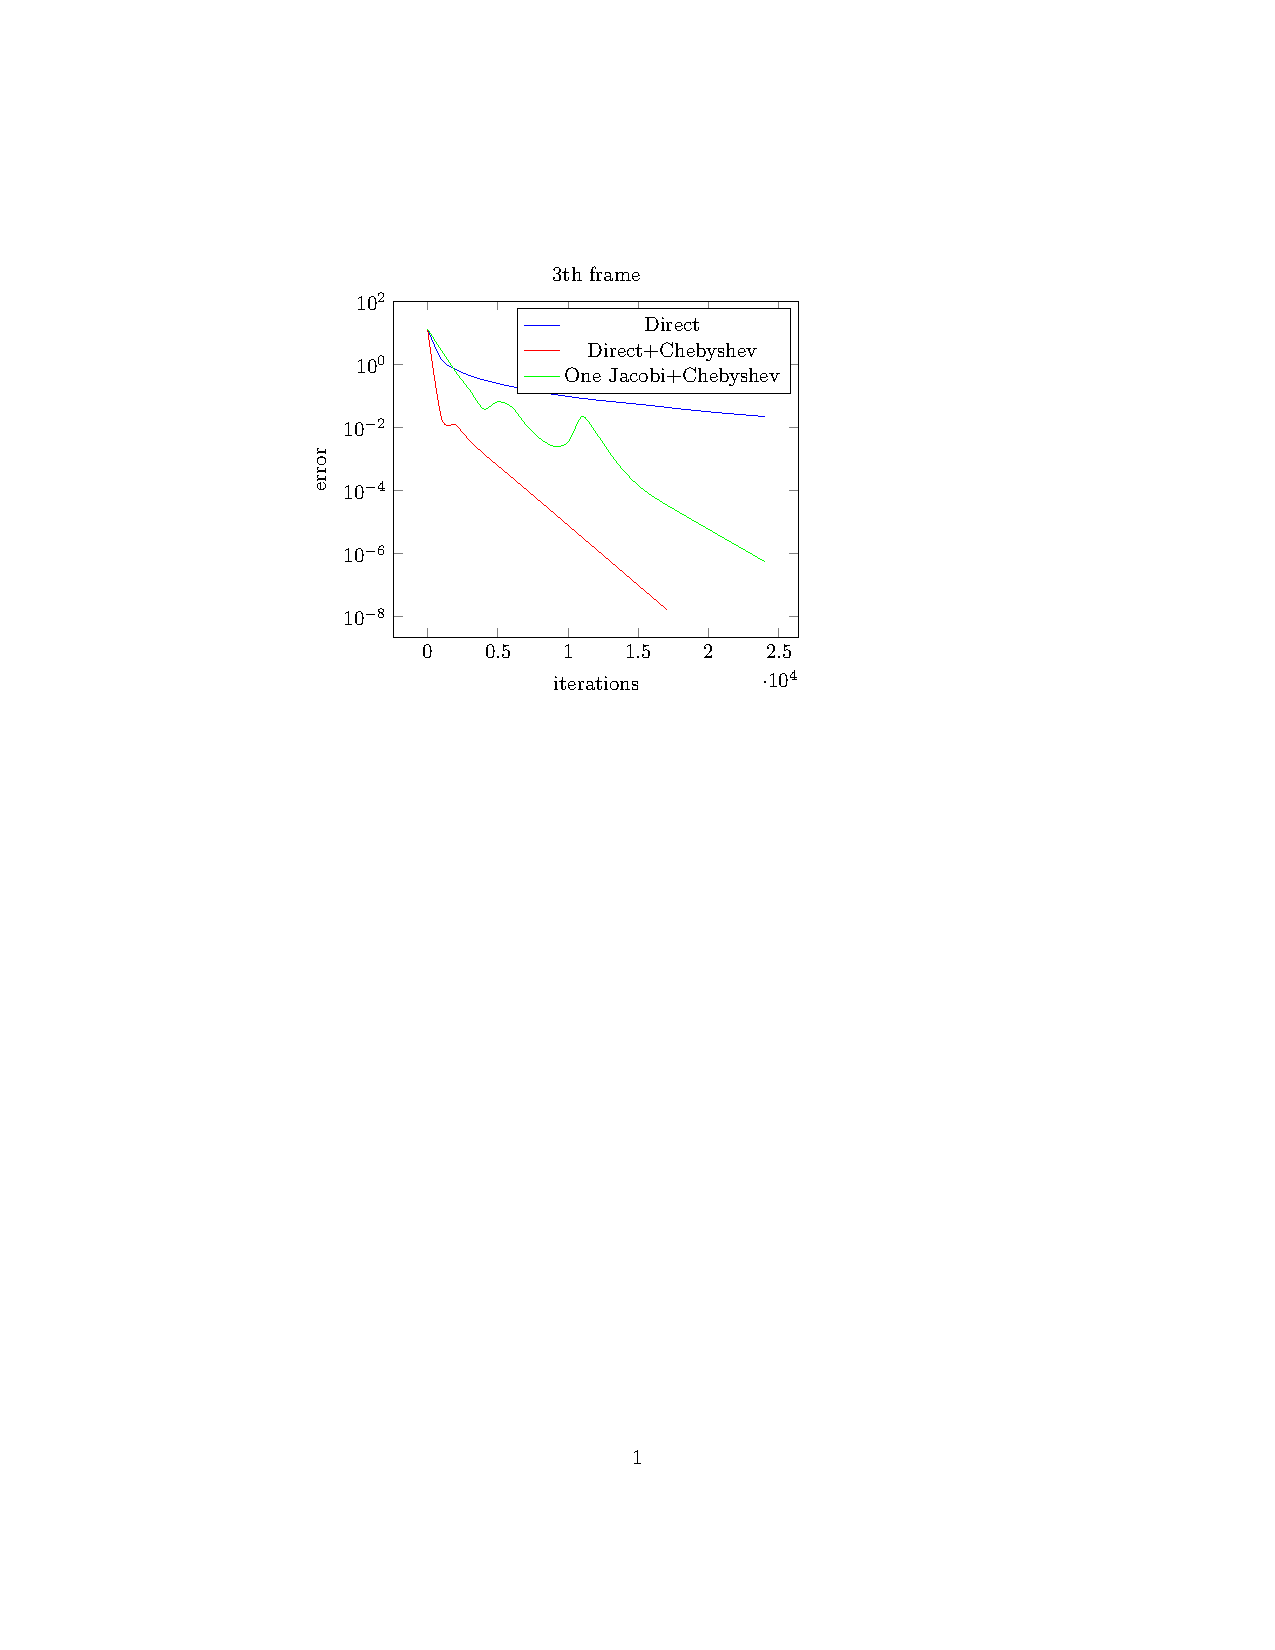
\includegraphics[scale=0.5]{img/plot}};
	\node at (2.5, -5) {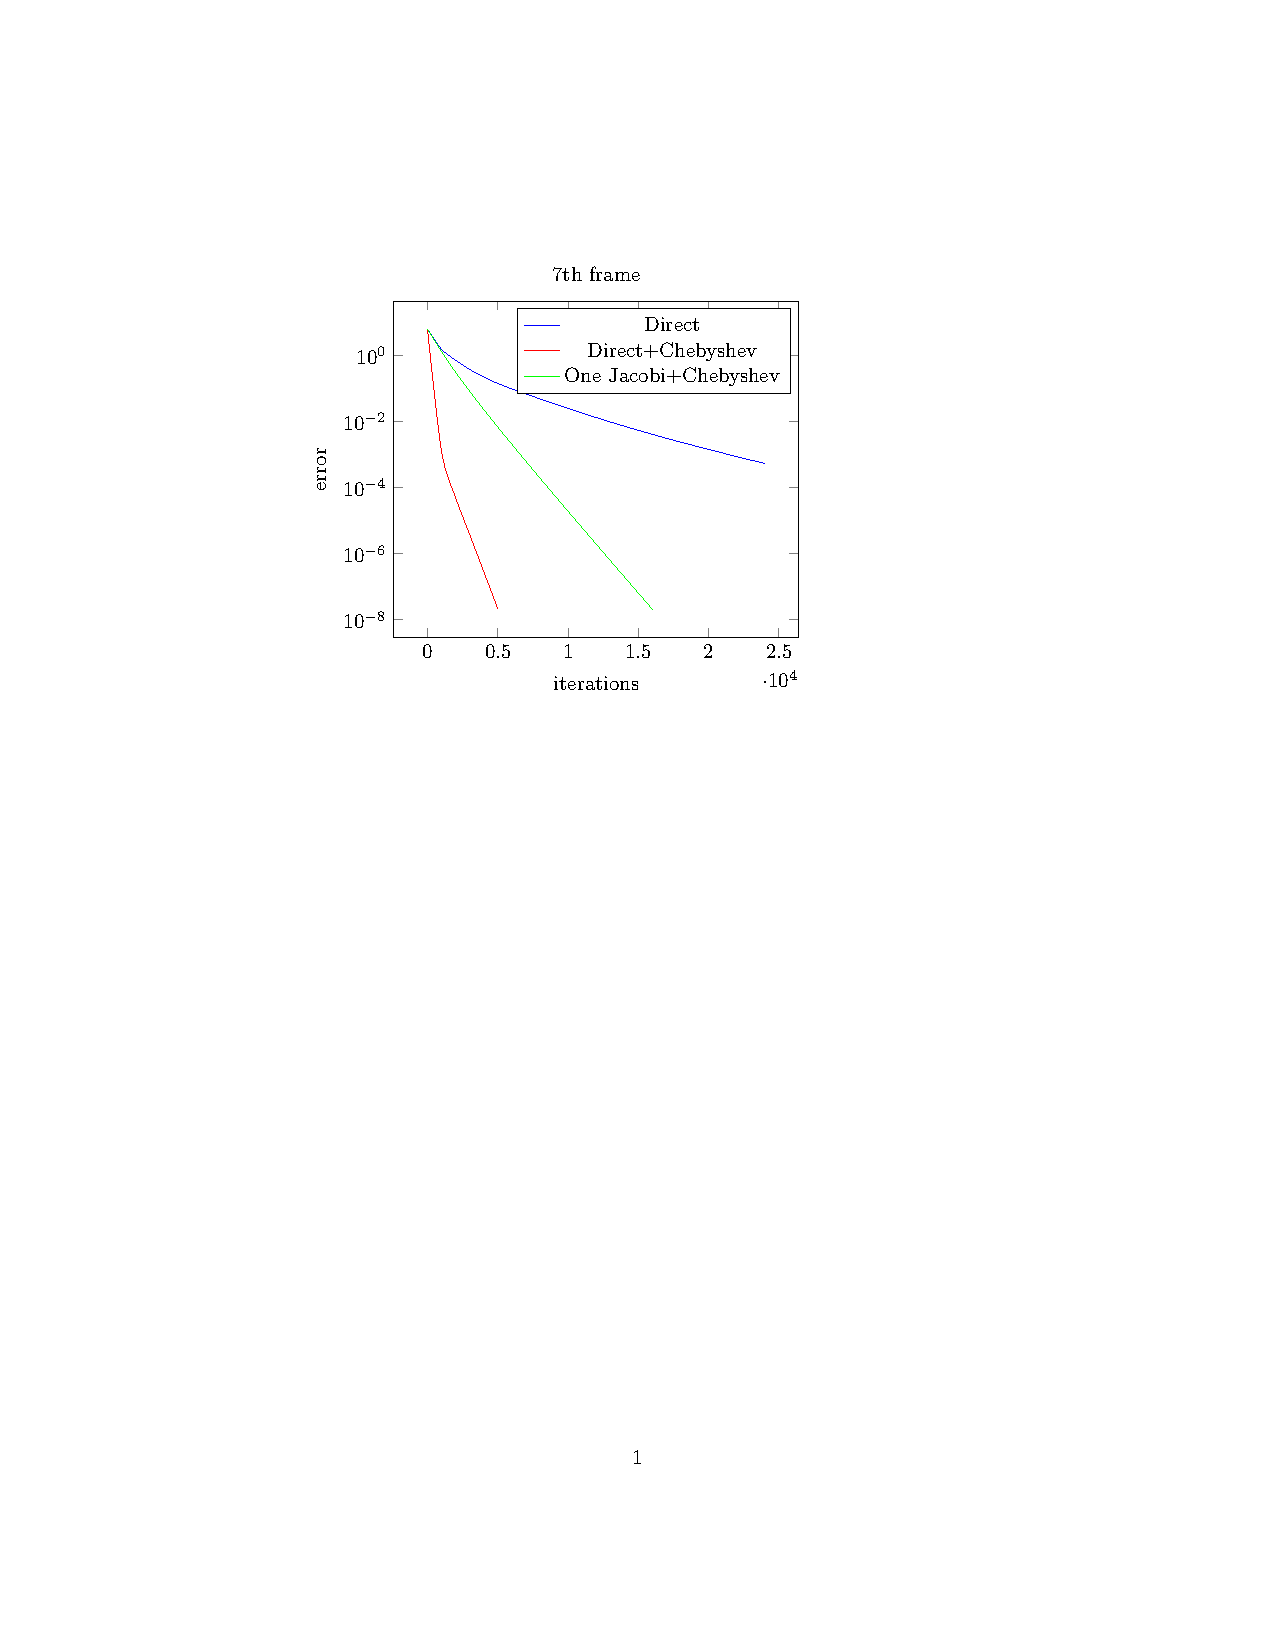
\includegraphics[scale=0.5]{img/plot1}};
      }
    }
    \pause
    \pause
    \item \TODOB{In mass spring, different approaches converged with a little different energy values.} 
  \end{itemize}
  %\gridlines
\end{frame}

\begin{frame}
 \frametitle{Comparison to CG}
 \TikzDraw {
  \node at (-2.4, -0.2) {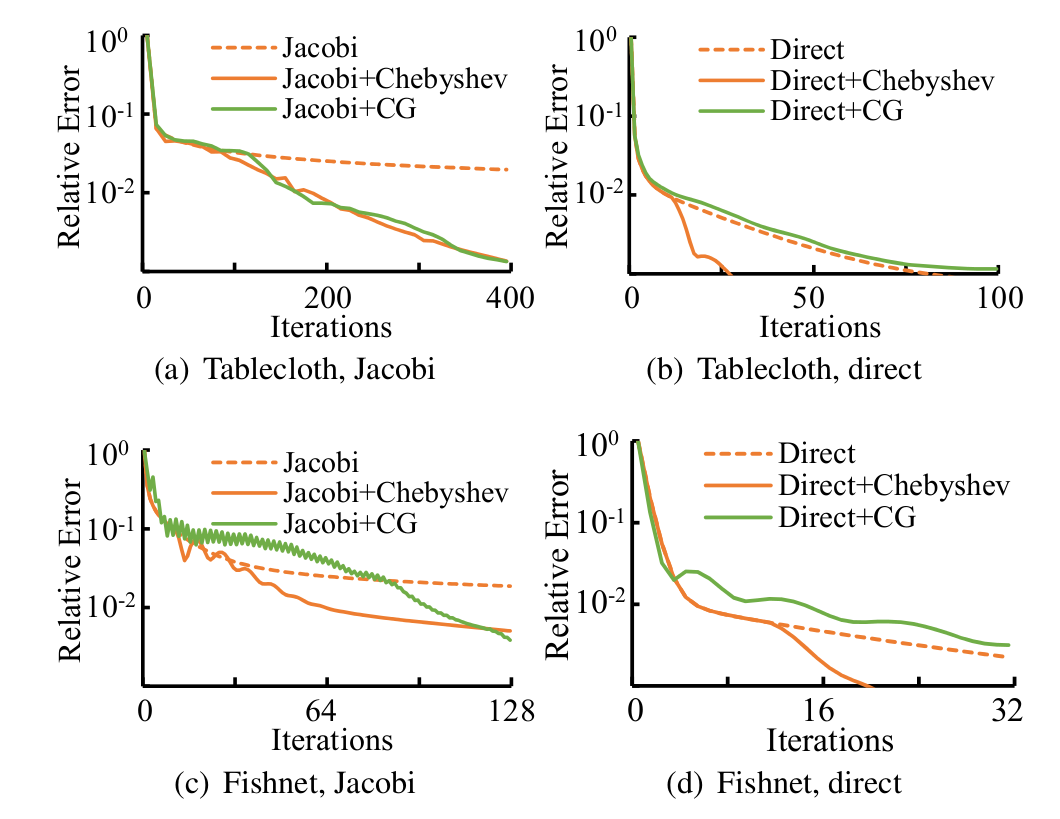
\includegraphics[scale=0.2]{img/cg_comp}};
  \node at (4.2, 0.1) {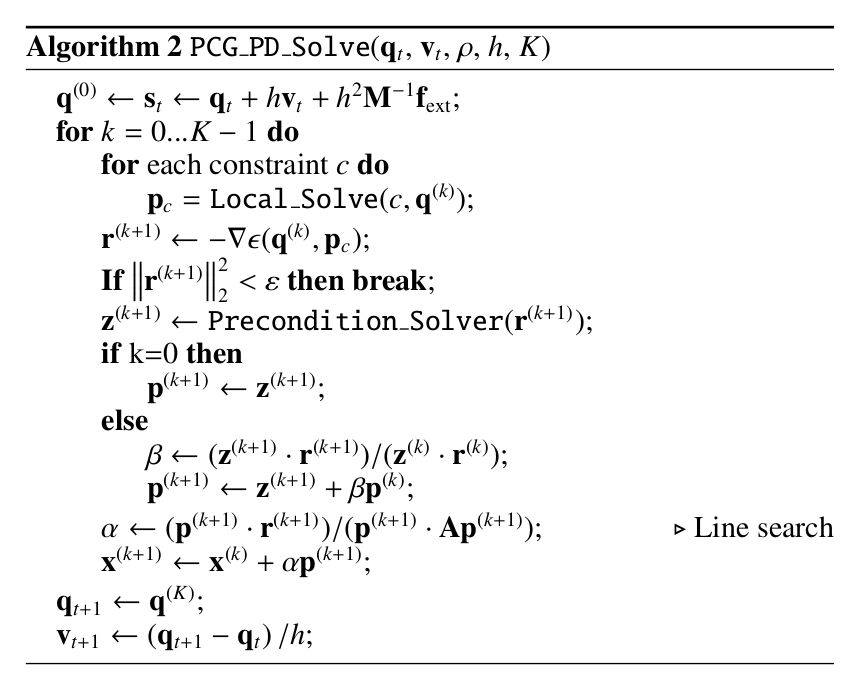
\includegraphics[scale=0.2]{img/cg}};
  \draw [fill=white, white] (5.6, -2.4) rectangle (6.4, 3);
  \draw [red, thick] (2.1, -1.05)--(4.12, -1.05);
 }
 %\gridlines
\end{frame}

\begin{frame}
 \frametitle{Conclusions}
 \textbf{Jacobi+Chebyshev}
 \begin{itemize}
  \item \TODO{Pros:}
  \begin{itemize}
   \item[-] Easy to implement, no requirement on linear solver libraries.
   \item[-] GPU friendly, small memory cost.
   \item[-] Relatively insensitive to small system changes, no need to re-factorize the matrix 
   when the system get changed.
  \end{itemize}
  \item \textcolor{green!50!black}{Cons:}
  \begin{itemize}
   \item[-] Sacrifice of robustness, divergence when mesh is in low quality or under large stress.
  \end{itemize}
 \end{itemize}
\end{frame}

\begin{frame} 
  \TikzDraw {
    \node at (0, 0.5) {\Huge{Thanks!}};
  }
\end{frame}

\end{document}
